%% question-1.tex
%%

%% ==============================
\subsection{Diagramme de classe minimaliste du jeu}
\label{sec:question-1}
%% ==============================

Voici, un diagramme de classe UML qui fixe les éléments principaux du jeu, c'est à dire le jeu en lui même, les lessons et les niveaux.

La classe principale Jeu possède une ou plusieurs lessons, ces lessons possèdent elles même un ou plusieurs niveaux.
Chaque niveau est le précédent ou le suivant d'un autre niveau.

\begin{figure}[h!]
	\centering
	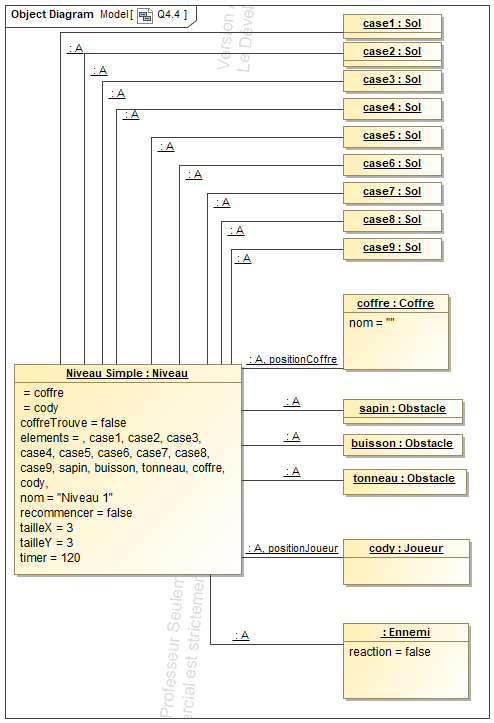
\includegraphics[width=250pt]{assets/Jeu_minimalist}
	\caption{Diagramme de classe des éléments principaux du jeu}
	\label{fig:diagrammeclassebase}
\end{figure}

\newpage